\documentclass[handout]{beamer}%[draft]
 \usepackage{beamerthemesplit}
 \usetheme{CambridgeUS}%Hannover
 \usecolortheme{dolphin}%dolphin
 %\setbeamercovered{transparent}
 \usepackage[utf8]{inputenc}
 %\usepackage{wsuipa}
 %\usepackage[ngerman]{babel}
 \usepackage{graphicx}
 \usepackage{multimedia}
 %\usepackage{media9}
 \usepackage{comment}
 \beamertemplatenavigationsymbolsempty
\usepackage{pgfpages}
\pgfpagesuselayout{4 on 1}[a4paper,border shrink=5mm]
 \title{Balltracking method}
 \author{Christian Gößl}
 \date{\today}
\begin{document}
\maketitle
\begin{frame}
	\frametitle{Structure}
	\tableofcontents
\end{frame}
	
\section{Motivation}
	
\frame[<+->]{
\frametitle{Motivation}
\begin{columns}
	\column{.5\textwidth}
	\begin{itemize}
	\item tracking photospheric flows of the surface of sun 
	\item method for evaluation and calculation of data from SOHO/MDI
	\end{itemize}
	\column{.5\textwidth}
	\begin{center} 
	\movie[width=5cm,height=5cm,poster,showcontrols,repeat]{}{gran_raw2.ogg}%,externalviewer
	%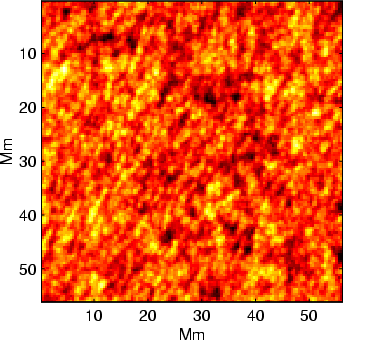
\includegraphics[scale=0.4]{img8_1.png}%height=7cm,width=4cm, 
	\end{center}
\end{columns}
}
	
	\section{Main idea}
	\begin{frame}\frametitle{Main Idea}
	\begin{center}
	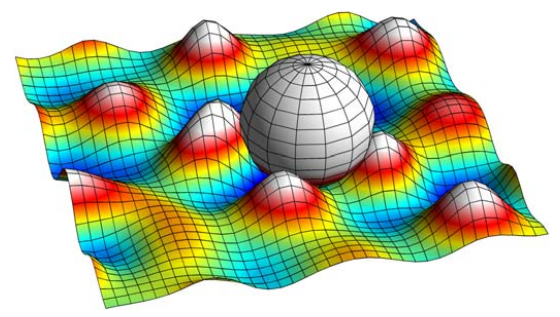
\includegraphics[scale=0.8]{floating_ball.png}
	\end{center}
	\end{frame}
	
	\frame[<+->]{

\begin{center} 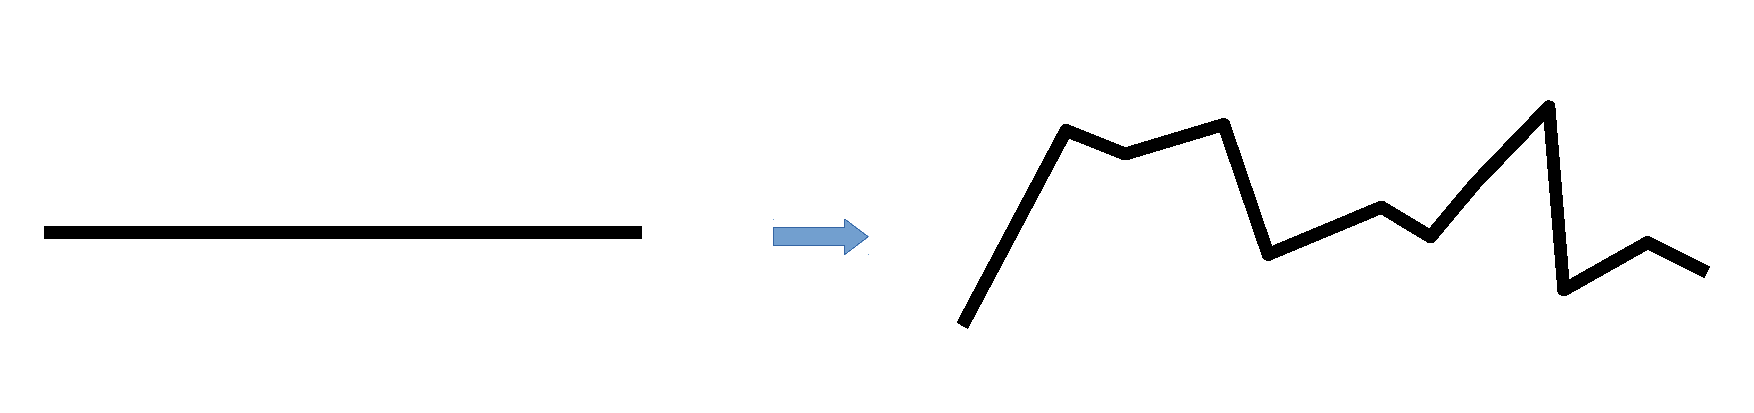
\includegraphics[scale=0.4]		{surface_1.pdf}%height=7cm,width=4cm, 
	\end{center}
	\begin{columns}
	\column{.5\textwidth}
	\begin{itemize}
	\item consist of bumps which moves(random walk), disappears and forming
	\item interaction between the bumps
	\item tracking the bumps with floating balls
	\end{itemize}
	\column{.5\textwidth}
	\begin{itemize}
	\item bumps push the balls 
	\item approx balls have the average motion/direction of the bumps
	\item prediction of mean motion of the bumps
	\end{itemize}
\end{columns}
}
	
	
	
	\begin{frame}
	\begin{center}	
	\movie[width=7cm,height=7cm,poster,showcontrols,repeat]{}{ball1.ogg}%,externalviewer
	%\fbox{\includemedia[width=7cm,height=7cm]{}{balls250sl.gif}}
	\end{center}
	\end{frame}
	
	\section{Tracking procedure}
	\subsection{Ball motion}
\frame[<+->]{%[label=Liste]
	\frametitle{Ball motion}
	\begin{center}
	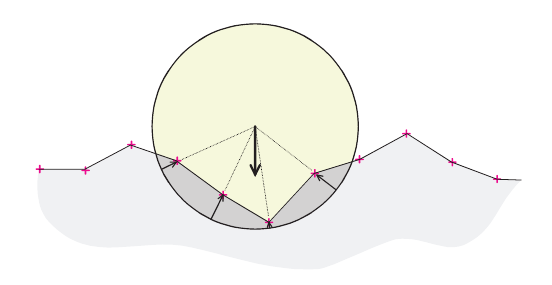
\includegraphics[scale=0.4]{penetration_ball.png}
	\hspace*{1cm}
	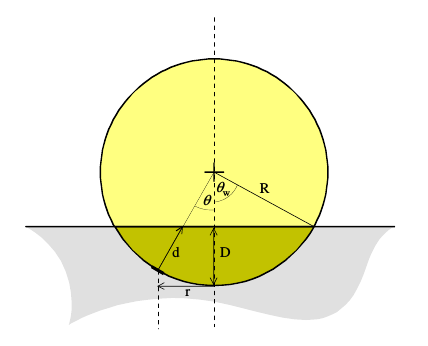
\includegraphics[scale=0.4]{sketch_ball_flat_surface.png}
	\end{center}
	\begin{columns}
	\column{.4\textwidth}
	\begin{itemize}
	\item $ m\dot{\vec{v}} = \sum_i \vec{f_i} - m\vec{g} -\alpha \vec{v} $		
	\item $ \vec{f_i} $ penetration force at each data points at the ball
	\end{itemize}
	\column{.6\textwidth}
	\begin{itemize}
	\item $ m\vec{g} $ gravitation force and $ -\alpha\vec{v} $ damping force
		\item $ d\vec{v} = dt\left( \frac{\stackrel{\thicksim}{A}_m}{\pi \stackrel{\thicksim}{D}_p^2\stackrel{\thicksim}{R}_s^2}\sum_i\stackrel{\thicksim}{d}_i - \stackrel{\thicksim}{A}_m \stackrel{\wedge}{g} - \frac{\vec{v}}{\stackrel{\thicksim}{T}_d}\right)$%  \diatop[a|a]
	\end{itemize}
	\end{columns}
}

\subsection{Steps to Analysing data}
\frame[<+->]{%[label=Liste]
	\frametitle{Steps to Analysing data}
	\begin{columns}
	\column{.5\textwidth}
	\begin{itemize}
	\item{1: choose number of balls
	\begin{itemize}
	\item  track every possible future
	\item  avoiding multiple balls that tracking the same feature 
	\end{itemize}}
	\item 2: divide data surface in a grid and randomly set balls in grid cells
	\item 3: let the balls  settle down to the nearest local minimum
	\item 4: update the surface to the next time step
	\end{itemize}
	\column{.5\textwidth}
	\begin{itemize}
	\item 5: bumps moving, disappearing, forming and pushed the balls to the next local minimum (store new position)
	\item 6: remove any balls which too close to each other balls and falling off the edge
		\item Repeat from Step 4 
	\end{itemize}
	\end{columns}
}
\subsection{Examples}
\begin{frame}
	\frametitle{Examples}
	\begin{center}	
	\movie[width=5cm,height=5cm,poster,showcontrols,repeat]{}{gran_raw2.ogg}%,externalviewer
	 \hspace{0.2cm}
		\movie[width=5cm,height=5cm,poster,showcontrols,repeat]{}{gran_filt2.ogg}%,externalviewer \fbox{}
	\end{center}
\end{frame}

\begin{frame}
\begin{center}	
\movie[width=7cm,height=7cm,poster,showcontrols,repeat]{}{grancork.ogg}%,externalviewer,autostart
\end{center}
\end{frame}

\begin{frame}
\begin{center}	
\movie[width=4cm,height=7cm,poster,showcontrols,repeat]{}{MDI_Balltracking2.ogg}%,externalviewer
\hspace{0.2cm}
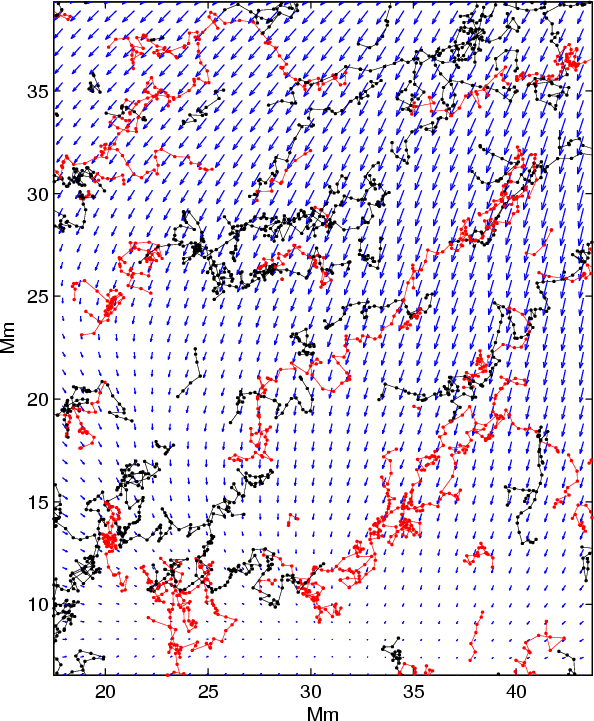
\includegraphics[scale=0.25]{img42.png}
\end{center}
\end{frame}

	\section{Further aspects}	
	\frame[<+->]{
	\frametitle{Further aspects}
	\begin{itemize}
	\item{ smoothing and rescaling the output data
	\begin{itemize}
		\item smoothing resolution
		\item speed calibration
	\end{itemize}}
	\item comparison between Local Correlation tracking LCT and Balltracking
	\end{itemize}
}
	
\section{Sources}	
\begin{frame}
	\frametitle{Sources}
	\begin{itemize}
	\item \url{http://www.astro.gla.ac.uk/users/hugh/balltrack/index.html}
	\item \url{http://www.aanda.org/articles/aa/abs/2004/34/aa0891/aa0891.html}
	\end{itemize}
\end{frame}
	
\end{document}